% ============================================================================
% CHAPTER 2 --- MACHINE LEARNING
% ============================================================================
\chapter{Machine Learning}
\label{ch:machine_learning}

Machine learning (ML) has emerged as a fundamental computational paradigm for extracting meaningful patterns from complex, high-dimensional data. Unlike traditional algorithmic approaches that rely on explicit, rule-based programming, ML models autonomously adapt their internal parameters to optimize performance on specific tasks based on data. Within the broader ML landscape, Artificial Neural Networks (ANNs), inspired by the biological architecture of the human brain, have demonstrated unprecedented success in modeling non-linear relationships. In other words, Machine Learning is a field that involves analyzing data to create mathematical models capable of generalizing unseen data.

This chapter outlines the theoretical foundations of the neural network architectures utilized in this research. It first formalizes the paradigms of supervised and unsupervised learning, detailing how neural networks operate under each framework. Subsequently, the chapter provides an in-depth examination of autoencoders, a specific class of neural networks uniquely suited for dimensionality reduction, feature extraction, and representation learning, which play a critical role in the methodology of this thesis.

\section{Supervised Learning in Neural Networks}
Supervised learning is a paradigm in which a model is trained on a labeled dataset. The primary objective is to learn a mapping function from input variables to an output variable, enabling the model to accurately predict the output for unseen, novel data~\cite{google_supervised}. In the context of this thesis, supervised learning is the core idea used hand in hand with SCF in Chapter~\ref{ch:nnscf}.

\begin{figure}[H]
    \centering
    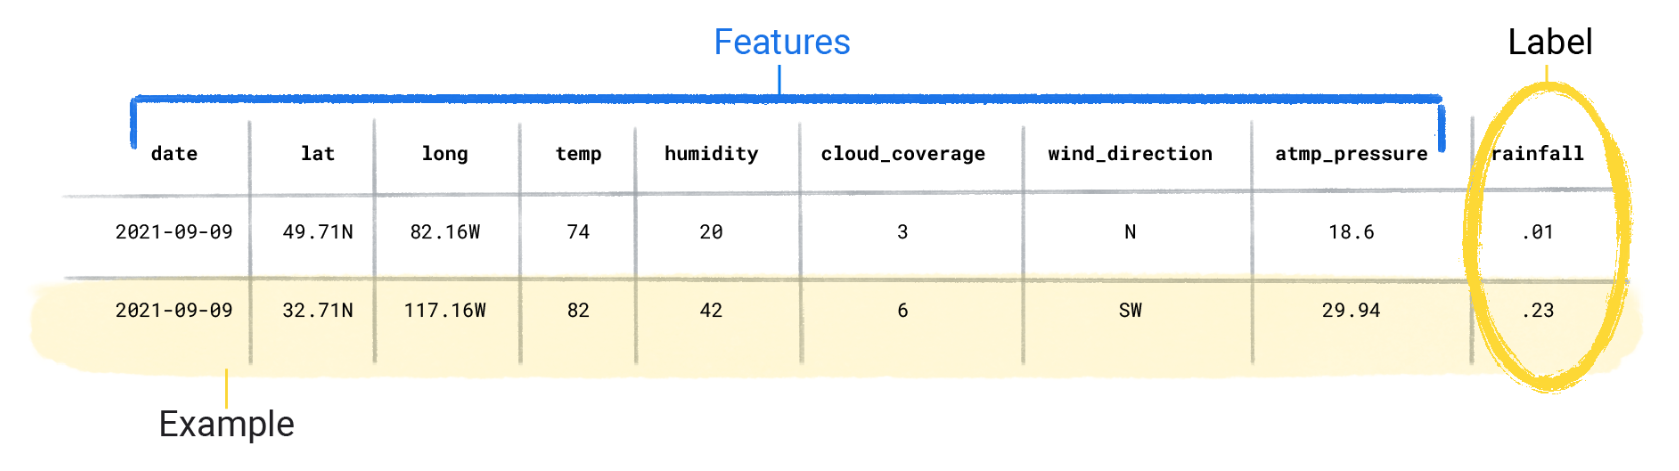
\includegraphics[width=0.95\textwidth]{Figures/Machine_Learning/Picture1.png}
    \caption{An example of a labeled dataset.}
    \label{fig:labeled_dataset}
\end{figure}

Formally, let $\mathcal{D} = \{(\mathbf{x}_i, y_i)\}_{i=1}^N$ represent a dataset of $N$ samples, where $\mathbf{x}_i \in \mathbb{R}^d$ is a $d$-dimensional input vector and $y_i$ is the corresponding ground-truth label or target value. A supervised neural network approximates a function $f(\mathbf{x}; \theta)$, parameterized by weights and biases denoted by $\theta$.

In a standard Feedforward Neural Network (FFNN), information propagates forward through hidden layers. The pre-activation output of a given layer $l$ is defined as:
\begin{equation*}
    \mathbf{z}^{(l)} = \mathbf{W}^{(l)} \mathbf{a}^{(l-1)} + \mathbf{b}^{(l)}
\end{equation*}
where $\mathbf{W}^{(l)}$ represents the weight matrix, $\mathbf{a}^{(l-1)}$ is the activation from the previous layer, and $\mathbf{b}^{(l)}$ is the bias vector. A non-linear activation function $\sigma$ (such as ReLU, Sigmoid, or Tanh) is then applied element-wise:
\begin{equation*}
    \mathbf{a}^{(l)} = \sigma(\mathbf{z}^{(l)})
\end{equation*}

The training process involves adjusting the parameters $\theta$ to minimize a predefined loss function $\mathcal{L}$, which quantifies the divergence between the network's predictions $\hat{y}_i = f(\mathbf{x}_i; \theta)$ and the true labels $y_i$. This is achieved through Empirical Risk Minimization (ERM):
\begin{equation*}
    \mathcal{J}(\theta) = \frac{1}{N} \sum_{i=1}^{N} \mathcal{L}(y_i, \hat{y}_i)
\end{equation*}

A loss function is used to compare between the ground-truth label and the model's prediction. Common loss functions include Mean Squared Error (MSE) for regression tasks and Cross-Entropy for classification tasks. The optimization of $\mathcal{J}(\theta)$ is typically performed using gradient-based methods, such as Stochastic Gradient Descent (SGD) or Adam, combined with the backpropagation algorithm, which efficiently computes the gradient of the loss function with respect to the network's weights via the chain rule of calculus.

\begin{figure}[H]
    \centering
    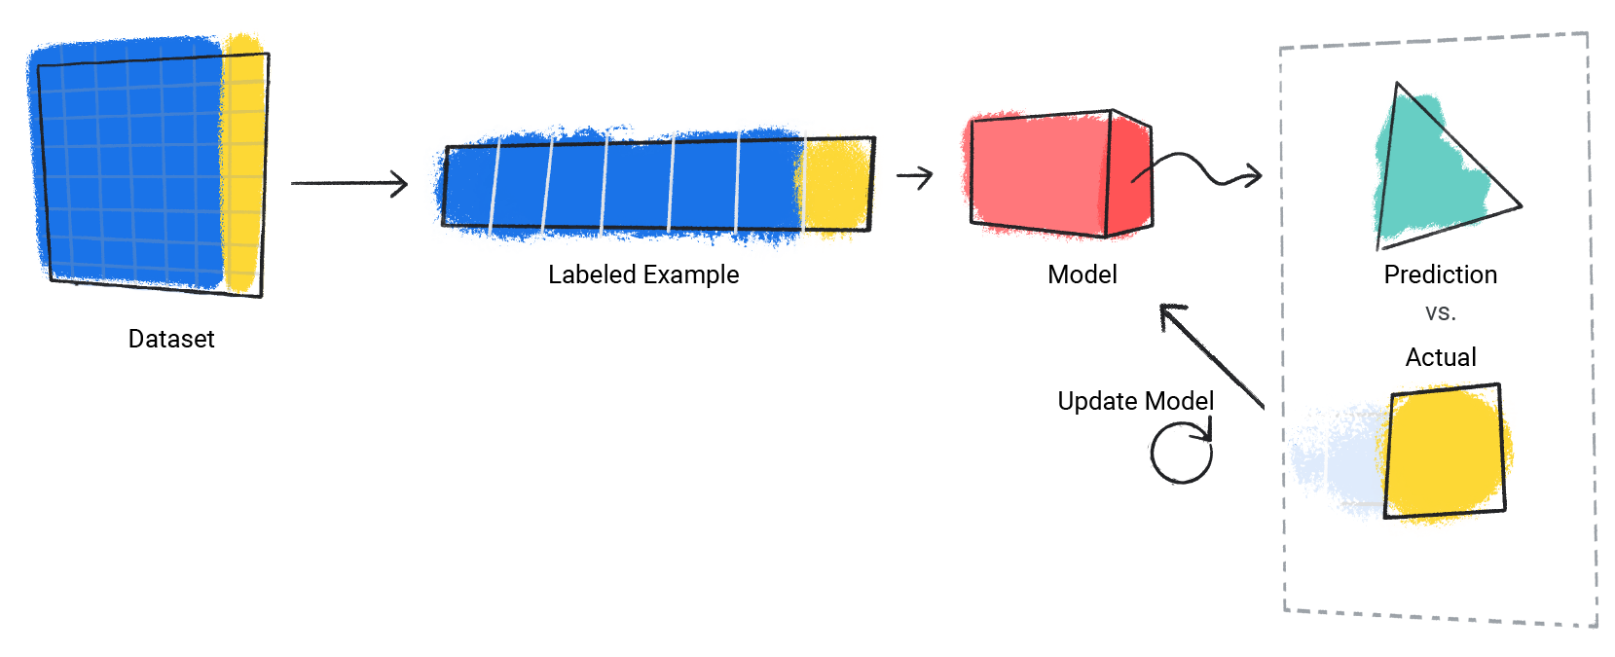
\includegraphics[width=0.75\textwidth]{Figures/Machine_Learning/Picture2.png}
    \caption{An ML model updating its predictions for each labeled example in the training dataset.}
    \label{fig:training_process}
\end{figure}

\section{Unsupervised Learning in Neural Networks}
In contrast to supervised learning, unsupervised learning involves training models on datasets that lack explicit labels or target outputs. The dataset is simply $\mathcal{D} = \{\mathbf{x}_i\}_{i=1}^N$. The primary objective here is to discover hidden structures, underlying distributions, or compressed representations within the data itself.

Unsupervised neural networks are instrumental in tasks such as clustering, anomaly detection, and generative modeling. By not relying on human-annotated labels, these models act as powerful exploratory tools. They attempt to model the underlying probability density $p(\mathbf{x})$ of the data or map the high-dimensional data manifold into a lower-dimensional subspace while preserving its topological properties. In the context of this thesis, unsupervised techniques are essential for the proposed technique related to tone reservation, as mentioned in Chapter~\ref{ch:dl_tr}.

\begin{figure}[H]
    \centering
    \begin{subfigure}[b]{0.48\textwidth}
        \centering
        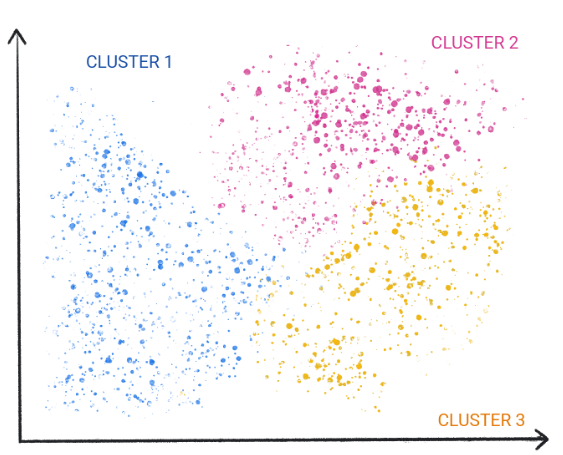
\includegraphics[width=\textwidth]{Figures/Machine_Learning/Picture3.png}
        \caption{An ML model clustering similar data points.}
        \label{fig:unsupervised_results}
    \end{subfigure}
    \hfill
    \begin{subfigure}[b]{0.48\textwidth}
        \centering
        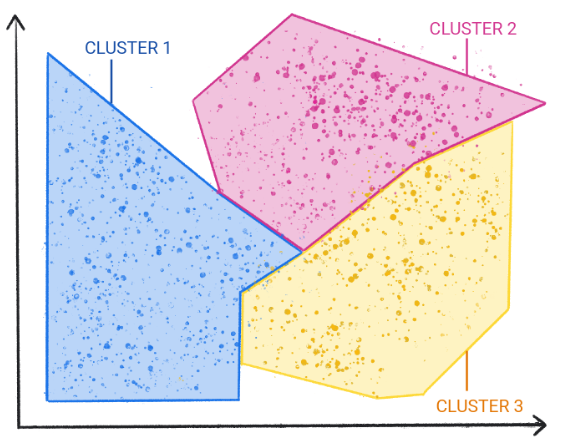
\includegraphics[width=\textwidth]{Figures/Machine_Learning/Picture4.png}
        \caption{Groups of clusters with natural demarcations.}
        \label{fig:actual_results}
    \end{subfigure}
    \caption{Illustration of unsupervised clustering.}
    \label{fig:unsupervised_vs_actual}
\end{figure}

\section{Artificial Neural Networks}
At its core, an Artificial Neural Network (ANN) is a computational model composed of interconnected processing units designed to recognize underlying relationships in a set of data. To understand how these models operate, whether in supervised or unsupervised paradigms, it is essential to define their structural and functional component. An easier way to look at it is to say that ANNs use the same structure of the neural networks in the human brain.

\begin{figure}[H]
    \centering
    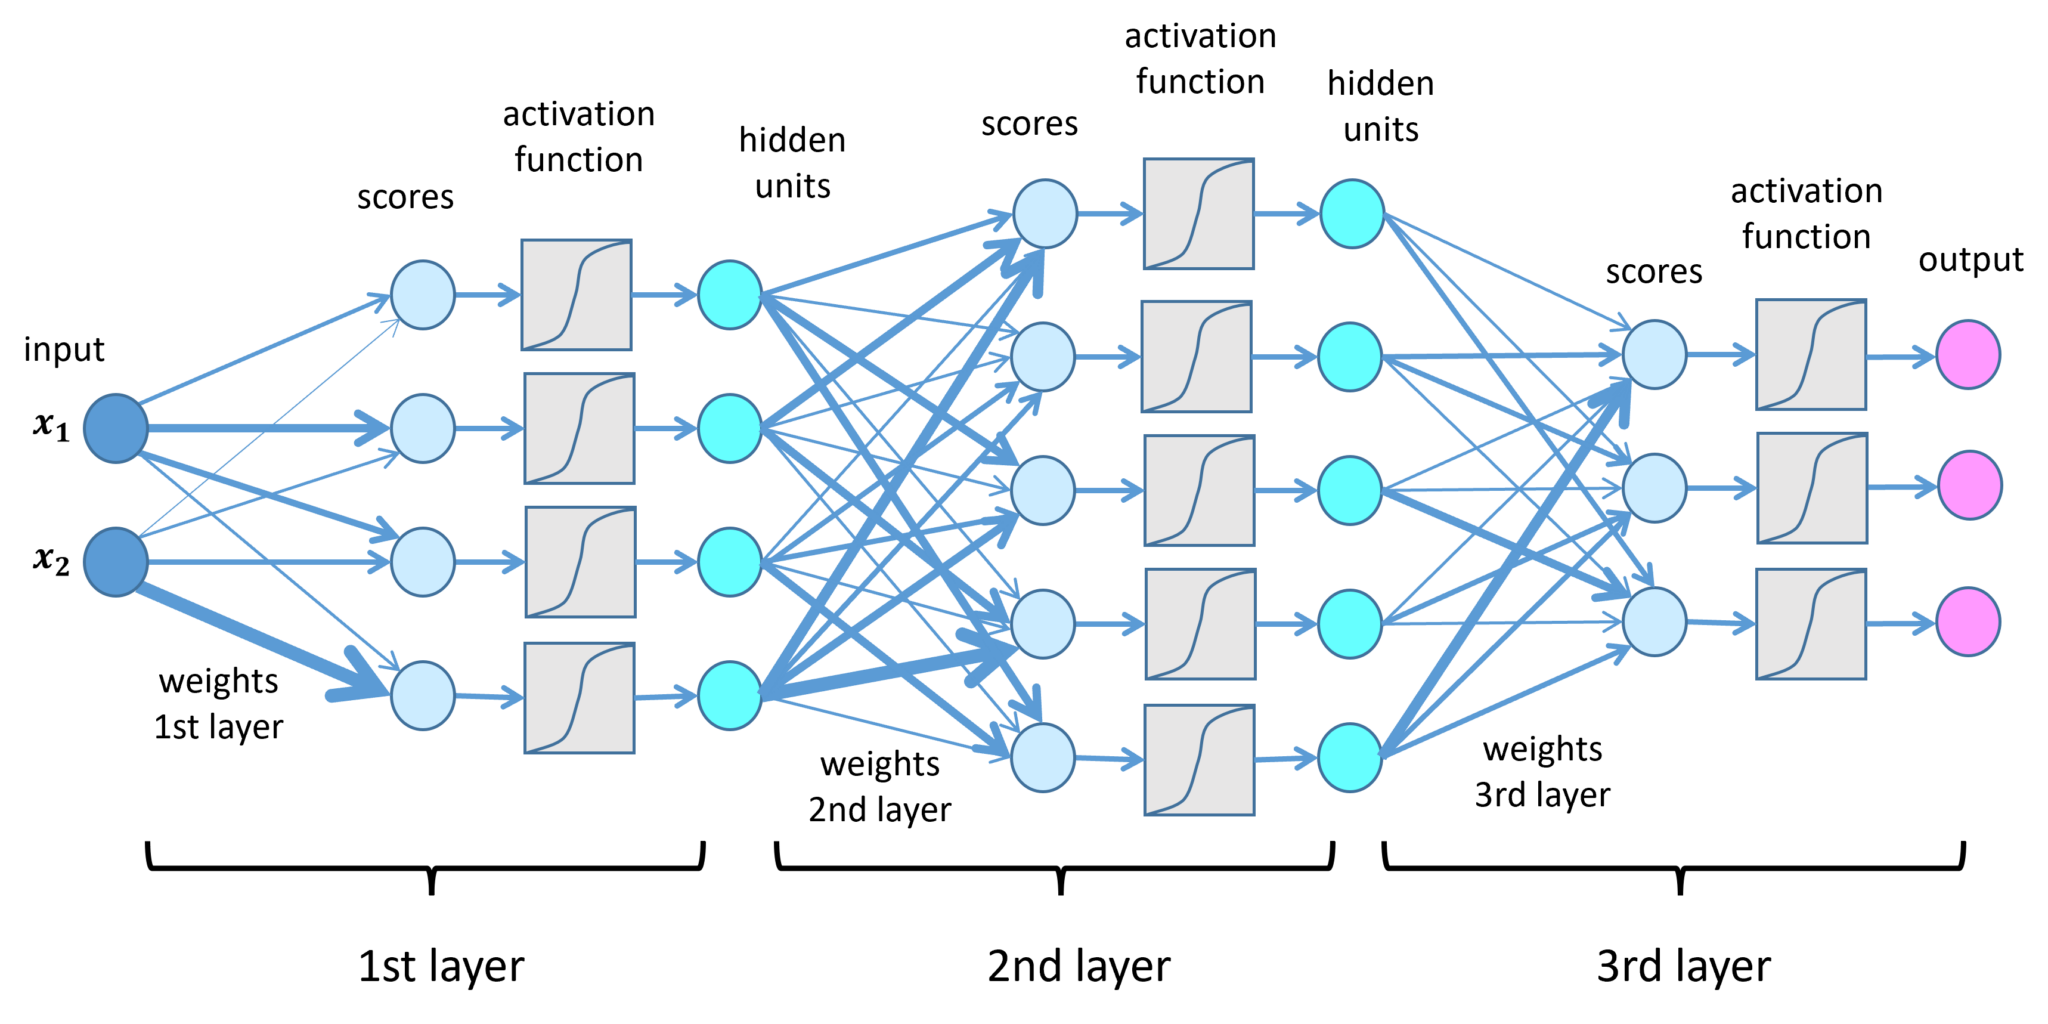
\includegraphics[width=0.9\textwidth]{Figures/Machine_Learning/deepLearn_2_EN-2048x1024.png}
    \caption{Structure of a Deep Neural Network}
    \label{fig:ann_structure}
\end{figure}

\subsection{Neurons}
The fundamental building block of an ANN is the artificial neuron, frequently referred to as a ``node.'' Inspired by biological neurons, these are the individual computational units within the network. Each node receives incoming signals---either raw data from the outside world or processed data from other nodes---aggregates them based on assigned weights, and determines an output signal to pass forward.

\subsection{Network Layers}
Nodes are not scattered randomly; they are organized into discrete, sequential stages called layers. The architecture of a standard feedforward neural network consists of three distinct layer types:

\begin{itemize}
    \item \textbf{The Input Layer:} This is the entry point for the dataset. Nodes in this layer do not perform any computations or apply activation functions; they simply hold the initial data values and pass them to the subsequent layer.

    \item \textbf{The Hidden Layers:} Situated between the input and output, hidden layers perform the heavy lifting of feature extraction and pattern recognition. A network may possess one hidden layer or multiple. As data traverses successive hidden layers, the network constructs increasingly complex, hierarchical representations of the data.

    \item \textbf{The Output Layer:} The final layer of the network, which synthesizes the processed information from the hidden layers into the desired target format (e.g., a continuous scalar for regression, a probability distribution for classification, or a reconstructed signal vector).
\end{itemize}

\subsection{Weights and Biases}
The flow of information between nodes is mediated by weights and biases, which together constitute the network's learnable parameters.

Weights dictate the strength or ``importance'' of a connection between a neuron in one layer and a neuron in the next. A near-zero weight effectively dampens an irrelevant input feature, while a large weight amplifies a critical one.

Biases act as scalar offsets applied to a neuron's aggregated input. Conceptually, a bias represents the threshold of activation for a given neuron, allowing the activation function to shift horizontally to better fit the underlying data distribution.

\subsection{Activation Functions}
Once a node aggregates its inputs, the resulting value is passed through an activation function before being transmitted to the next layer. The primary purpose of the activation function is to introduce non-linearity into the network. Without non-linear activation functions, an ANN, regardless of how many hidden layers it contains, would behave essentially as a single-layer linear regression model, incapable of solving complex, real-world problems.

\subsection{Backpropagation and Learning}
While the feedforward process generates a prediction, the actual ``learning'' occurs through an algorithm known as backpropagation (backward propagation of errors). During training, the network's output is compared against the desired target, and the discrepancy is quantified by a loss function. Backpropagation is the mechanism used to calculate the gradient of this loss function with respect to every weight in the network. By propagating the error backward from the output layer to the input layer, the network identifies how much each individual node contributed to the overall error. This allows optimization algorithms to systematically adjust the connections, iteratively improving the network's accuracy over time.

\section{Autoencoders}
An autoencoder is a specialized architecture of an artificial neural network designed to learn efficient data encodings. Belonging to the unsupervised learning paradigm (often referred to as self-supervised learning), its primary objective is not simply to duplicate data, but to learn how to compress it into a highly efficient, low-dimensional summary, and subsequently reconstruct the original data from that summary~\cite{wiki_autoencoder}. This concept is fundamentally present in PRNet's and RVNN's architectures in Chapters~\ref{ch:prnet} and~\ref{ch:rvnn} respectively.

\begin{figure}[H]
    \centering
    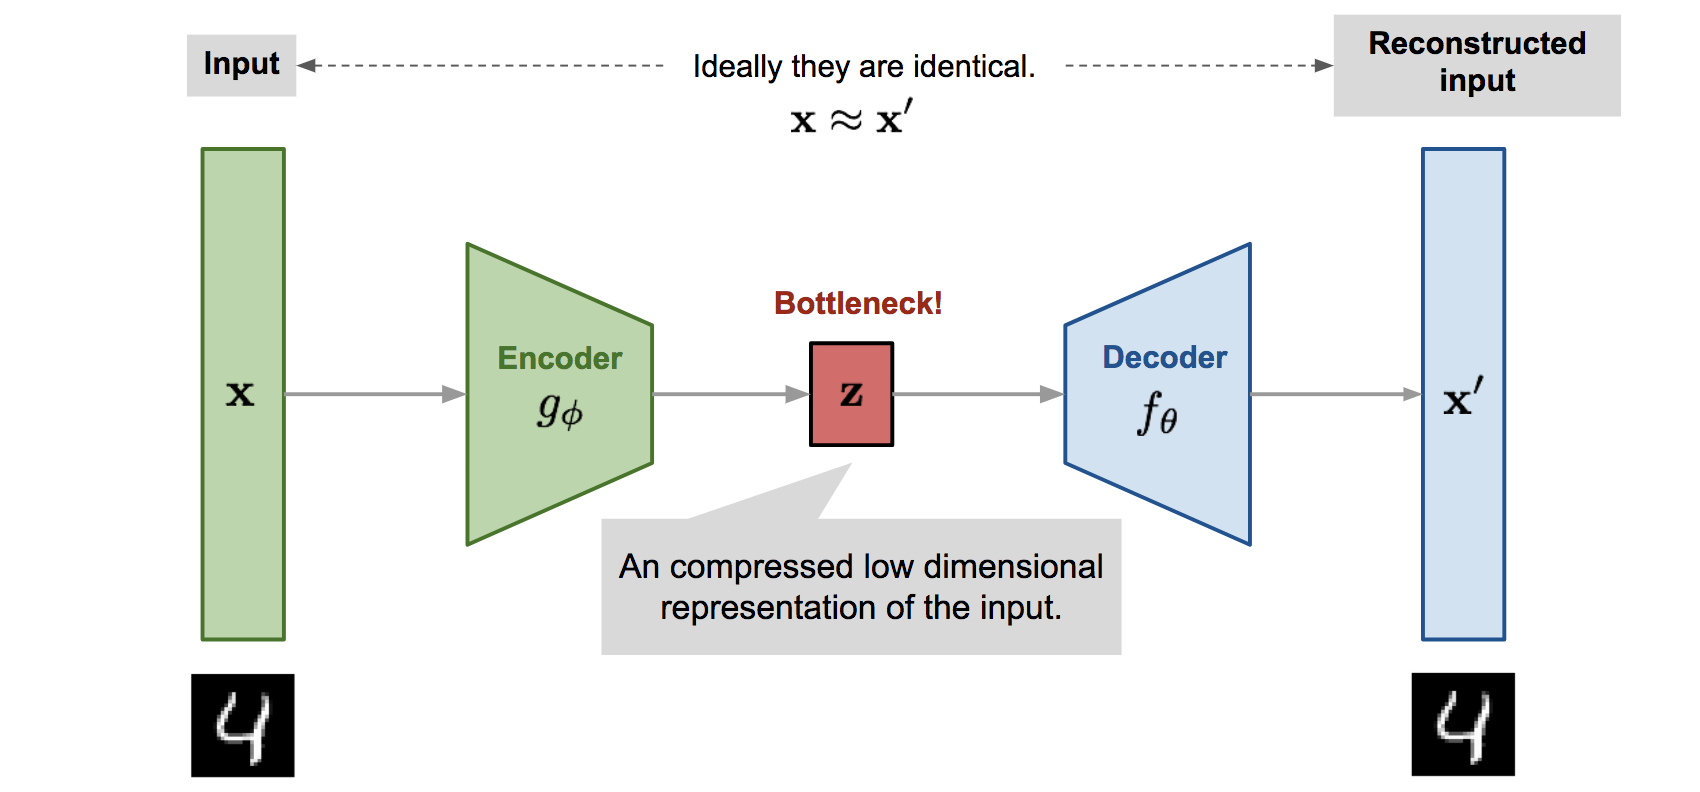
\includegraphics[width=0.8\textwidth]{Figures/Machine_Learning/autoencoder-architecture.png}
    \caption{Architecture of a standard autoencoder, illustrating the Encoder, Latent Space bottleneck, and Decoder.}
    \label{fig:autoencoder}
\end{figure}

The structure of an autoencoder is distinctively symmetrical and can be divided into three primary components:

\textbf{The Encoder:} This initial section of the network, denoted as $\mathbf{h} = f(\mathbf{x}; \phi)$, takes the original, high-dimensional input data $\mathbf{x} \in \mathbb{R}^d$ (such as a time-domain signal or an image) and progressively compresses it through a series of shrinking hidden layers into a hidden representation $\mathbf{h} \in \mathbb{R}^k$, where typically $k \ll d$. It acts as a mathematical funnel, extracting the most vital features while stripping away background noise and redundant information. The mapping is given by:
\begin{equation*}
    \mathbf{h} = \sigma(\mathbf{W} \mathbf{x} + \mathbf{b})
\end{equation*}
where $\phi = \{\mathbf{W}, \mathbf{b}\}$ are the encoder parameters.

\textbf{The Bottleneck (Latent Space):} Situated at the exact center of the network, this is a highly compressed, low-dimensional representation of the input data. By forcing the information through this heavily restricted bottleneck, the network is compelled to retain only the absolute most essential, defining characteristics of the original input. In the context of end-to-end telecommunication machine learning models, this latent space is frequently used to mathematically represent the physical wireless channel.

\textbf{The Decoder:} This final section operates in reverse. The decoder network, denoted as $\hat{\mathbf{x}} = g(\mathbf{h}; \psi)$, takes the compressed data from the bottleneck and attempts to decompress the latent representation $\mathbf{h}$, mapping it back through expanding hidden layers to reconstruct the original high-dimensional input at the output layer as accurately as possible, producing $\hat{\mathbf{x}} \in \mathbb{R}^d$. The reconstruction mapping is formulated as:
\begin{equation*}
    \hat{\mathbf{x}} = \sigma'(\mathbf{W}' \mathbf{h} + \mathbf{b}')
\end{equation*}
where $\psi = \{\mathbf{W}', \mathbf{b}'\}$ are the decoder parameters.

\textbf{Training and Reconstruction Loss:}
Because an autoencoder uses its own input as the target output, it does not require pre-calculated, human-labeled datasets. During the training phase, the network systematically calculates the difference between its final reconstructed output $\hat{\mathbf{x}}$ and the original input $\mathbf{x}$. This discrepancy is quantified by a specialized loss function known as the reconstruction loss. For continuous data, the Mean Squared Error (MSE) is frequently utilized:
\begin{equation*}
    \mathcal{L}_{REC}(\phi, \psi) = \frac{1}{N} \sum_{i=1}^{N} ||\mathbf{x}_i - g(f(\mathbf{x}_i; \phi); \psi)||^2
\end{equation*}

Using the backpropagation algorithm, the network continuously adjusts its internal weights across both the encoder and decoder to minimize this loss, ensuring that the reconstructed output matches the original input with the highest possible fidelity. In this research, autoencoders are deployed to find a non-linear mapping from input data to a low-PAPR sequence that can be accurately reconstructed.
